\section{Solving Non-linear Real Arithmetic formulas with Virtual Substitution}
\label{sec:solving non-linear equalities with virtual substitution}
\subsection{Test Candidates and Side Conditions}
Let $p(x) = ax^{2} + bx + c$ is a quadratic of variable $x$ where $p \in P$ and $a, b, c$ do not contain $x$. We assume $p(x) \sim 0, \sim \in \{=,<,>,\leq,\geq,\neq\}$. Now, the solution equations for $x$ in $p(x)$ considers the following four cases:
\begin{alignat}{2}
	&x_{0} = -\frac{c}{b}\qquad                            
	&& \text{, if $ a = 0 \wedge b\neq 0$} \\
	&x_{1} = \frac{-b + \sqrt{b^{2}-4ac}}{2a}\qquad      
	&& \text{, if $ a \neq 0 \wedge b^{2}-4ac\geq 0$} \\
	&x_{2} = \frac{-b - \sqrt{b^{2}-4ac}}{2a}\qquad      
	&& \text{, if $ a \neq 0 \wedge b^{2}-4ac\geq 0$} \\
	&x_{3} = -\infty\qquad      
	&& \text{, if $ a = 0 \wedge b = 0$}
\end{alignat}
Here $x_{0}, x_{1}, x_{2}$ and $x_{3}$ are the real zeros of $p$ in $x$ and the conditions on the right are called side conditions.\newline
The constraint $p(x) \sim 0$ has solution intervals $(-\infty, x_{0})$ or $(x_{i}, x_{i+1})$or $[x_{i}, x_{i}]$or $([x_{2}, x_{2}]$ or $(x_{2}, \infty)$ where $0\leq i\leq 1$. So, the endpoints of these intervals are $-\infty, x_{i}$ and $x_{2}$ which are the real zeros. As the real zeros are symbolic and we cannot order them to pick the solutions. Hence, we choose a left endpoint of each left closed interval, a left endpoint of each left opened interval plus an infinitesimal $\epsilon$ as sample solutions shown in the Figure \ref{fig:testcandidates}. These sample solutions are called test candidates.
\begin{center}
	\begin{figure}[!h]
\centering
\begin{tikzpicture}[scale=0.6,line cap=round,line join=round,>=triangle 45,x=1.0cm,y=0.1cm]
\draw[-,color=black] (-4.3,0.) -- (18.7,0.);
\foreach \x in {-4.,-3.,-2.,-1.,1.,2.,3.,4.,5.,6.,7.,8.,9.,10.,11.,12.,13.,14.,15.,16.,17.,18.}
\draw[shift={(\x,0)},color=black] (0pt,-2pt);
\clip(-4.3,-5.34) rectangle (18.7,6.3);
\begin{scriptsize}

\draw[color=black] (-3.90,-3) node {$-\infty$};
\draw [color=black] (-4.0661824267070554,0.)-- ++(-2.5pt,-2.5pt) -- ++(5.0pt,5.0pt) ++(-5.0pt,0) -- ++(5.0pt,-5.0pt);

\draw[color=black] (3.5,-3) node {$x_{0}$};
\draw [color=black] (3.5,0.)-- ++(-2.5pt,-2.5pt) -- ++(5.0pt,5.0pt) ++(-5.0pt,0) -- ++(5.0pt,-5.0pt);

\draw[color=black] (3.8,3) node {$x_{0}+\epsilon$};
\draw [color=black] (3.8,0.)-- ++(-2.5pt,-2.5pt) -- ++(5.0pt,5.0pt) ++(-5.0pt,0) -- ++(5.0pt,-5.0pt);

\draw[color=black] (7.00,-3) node {$x_{1}$};
\draw [color=black] (7.00,0.)-- ++(-2.5pt,-2.5pt) -- ++(5.0pt,5.0pt) ++(-5.0pt,0) -- ++(5.0pt,-5.0pt);

\draw[color=black] (7.30,3) node {$x_{1}+\epsilon$};
\draw [color=black] (7.30,0.)-- ++(-2.5pt,-2.5pt) -- ++(5.0pt,5.0pt) ++(-5.0pt,0) -- ++(5.0pt,-5.0pt);


\draw[color=black] (10.50,-3) node {$x_{2}$};
\draw [color=black] (10.50,0.)-- ++(-2.5pt,-2.5pt) -- ++(5.0pt,5.0pt) ++(-5.0pt,0) -- ++(5.0pt,-5.0pt);

\draw[color=black] (10.8,3) node {$x_{2}+\epsilon$};
\draw [color=black] (10.8,0.)-- ++(-2.5pt,-2.5pt) -- ++(5.0pt,5.0pt) ++(-5.0pt,0) -- ++(5.0pt,-5.0pt);

\draw[color=black] (18.24,-3) node {$\infty$};
\draw [color=black] (18.50,0.)-- ++(-2.5pt,-2.5pt) -- ++(5.0pt,5.0pt) ++(-5.0pt,0) -- ++(5.0pt,-5.0pt);

\end{scriptsize}
\end{tikzpicture}
\caption{Test Candidates}
\label{fig:testcandidates}
\end{figure}
\end{center}
To solve a non-linear real arithmetic formula $\varphi$, first we have to choose a variable $x, x\in p(x)$ to eliminate and then compute all possible test candidates of $x$. $\varphi$ is satisfiable if there is a test candidate $t\in T$ such that $\varphi [t\backslash\backslash x] = p_1[t\backslash\backslash x] \wedge \cdots p_n[t\backslash\backslash x] \wedge side Condition$ is satisfiable, but direct substitution is not possible as test candidates are not algebraic $(\sqrt\text{ }, \epsilon, -\infty, \%,\ldots )$. Thus, virtual substitution rules need to be introduced.
\subsection{Virtual Substitution}
Virtual substitution is a procedure to eliminate a quantified variable. Let $\varphi$ be a quantifier-free real arithmetic formula where $x\in p(x)$ and $p(x) \sim 0, \sim \in \{=,<,>,\leq,\geq,\neq\}$ is a constraint of   $\varphi^\mathbb{R}$. Degree of $x$ in $p(x)$ must be at most two. Then, quantifier elimination by virtual substitution is based on the following equivalence:
$$ \exists x\varphi \Longleftrightarrow \bigvee\limits_{t\in T(x,\varphi)}  (\varphi [t\backslash\backslash x] \wedge C_t)$$
Where $T$ is a finite set of all possible test candidates for $x$ and $C_t$ is a side condition of test candidate $t \in T$.

Virtual Substitution is a restricted but very efficient procedure to solve non-linear equalities. In the paper [1] author explored an extension of the ideas in [2] from the linear to the quadratic case. For linear case the idea was to eliminate a quantifier from $\exists x \varphi$ by replacing $x$ in $\varphi$ with $t$ that may involve improper expressions such as $\pm \infty$ or $\epsilon$. However, $\varphi [t\backslash\backslash x]$ is defined in such a way that these improper expressions do not occur in the resulting formula.

Author extended these idea to various quadratic cases. The cases are the substitution of square root expressions and the substitution of infinitesimal expressions in formulas.

In virtual substitution, first a variable is replaced by test candidate and to perform the replacement we need to construct test candidates. An univariate real-arithmetic formula is satisfiable if and only if there is one test candidate for which satisfies formula and the side conditions of t holds. For multivariate real-arithmetic formula the virtual substitution method continues with the elimination of the next variable.
\subsection{Constructing test candidates with side condition}
Let a quadratic equation $p(x) = p_{1}x^{2} + p_{2}x + p_{3} = 0$ in the variable $x$ where $p_{1}, p_{2}, p_{3} \in P$ and $x$ does not contain in $p_{1}, p_{2}$ and $p_{3}$. Now, we get the solution formula for $x$ in $p(x)$ as follows:
\begin{alignat}{2}
	&x_{0} = -\frac{p_{3}}{p_{2}}\qquad                            
	&& \text{, if $ p_{1} = 0 \wedge p_{2}\neq 0$} \\
	&x_{1} = \frac{-p_{2} + \sqrt{p_{2}^{2}-4p_{1}p_{3}}}{2p_{1}}\qquad      
	&& \text{, if $ p_{1} \neq 0 \wedge p_{2}^{2}-4p_{1}p_{3}\geq 0$} \\
	&x_{2} = \frac{-b - \sqrt{p_{2}^{2}-4p_{1}p_{3}}}{2a}\qquad      
	&& \text{, if $ p_{1} \neq 0 \wedge p_{2}^{2}-4p_{1}p_{3}\geq 0$} \\
	&x_{3} = -\infty\qquad      
	&& \text{, if $ p_{1} = 0 \wedge p_{2} = 0 \wedge p_{3}=0$}
\end{alignat}
Here $x_{0}, x_{1}$ and $x_{2}$ are the symbolic zeros of $x$ in $p(x)$.
\begin{definition}[Square Root Expression]
	\label{def:square root expression}
	A square root expression has the following form:
	$$\frac{p+q\sqrt{r}}{s}\qquad  \text{, where } p,q,r,s \in P $$
	and the set of all square root expression is denoted as follows:
	$$SqrtEx=\{\frac{p+q\sqrt{r}}{s}|\text{ }p,q,r,s\in P\} $$
	\begin{table}[htb]
		\bigskip % Insert a vertical space. Also \smallskip or \medskip.
		\begin{center}
			\begin{tabular}{|c|c|c|c|c|}
				\hline
				Equation No.& p & q & r & s \\
				\hline
				$2.1$ & $-p_{3}$ & $0$ & $1$ & $p_{2}$ \\
				\hline
				$2.2$ & $-p_{2}$ & $1$ & $p_{2}^{2}-4p_{1}p_{3}$ & $2p_{1}$ \\
				\hline
				$2.3$ & $-p_{2}$ & $-1$ & $p_{2}^{2}-4p_{1}p_{3}$ & $2p_{1}$ \\
				\hline
			\end{tabular}
		\end{center}
		\caption{Comparison with square root expression $\frac{p+q\sqrt{r}}{s}$}
		\label{sqrt}
	\end{table}
\end{definition} 
Now, we can express the symbolic zero of $x$ in $p(x)$, which is quadratic in x by a square root expression $\frac{p+q\sqrt{r}}{s}$ as given in Table \ref{sqrt}.\newline
So, for $x$ in $p(x)$, $SqrtEx=\{-\frac{p_{3}}{p_{2}}, \frac{-p_{2}\pm \sqrt{p_{2}^{2}-4p_{1}p_{3}}}{2p_{1}}\}$. Now, We can construct the set of all test candidates for $x$ in $p(x)\sim 0$ in terms of $SE\in SqrtEx$ which is given as follows:
		$$
		t
\quad = \quad 
\left\{
\begin{array}{ll}
{\displaystyle \{-\infty,SE} 
& 
\text{, if }\sim \text{ is weak }
\\[0.6cm] % adjust the line spacing
{\displaystyle \{-\infty,SE+\epsilon\}}
& 
\text{, otherwise }
\end{array}
\right.$$
Here weak means $\{=,\leq,\geq\}$.\newline
And the side condition of each test candidate $t$ is defined by:
		$$
C_t
\quad = \quad 
\left\{
\begin{array}{lll}
{\displaystyle C_{t^{\prime}}}
& 
\text{, if } t = t^{\prime} + \epsilon
\\[0.6cm] % adjust the line spacing
{\displaystyle \{s\neq 0 \wedge r\geq 0\}}
& 
\text{, if } t = \frac{p+q\sqrt{r}}{s}
\\[0.6cm] % adjust the line spacing
{\displaystyle true}
& 
\text{, Otherwise }
\end{array}
\right.$$
Here $t^{\prime}$ is a test candidate which does not contain $\epsilon$.\newline
Each side condition of the test candidates confirms that each test candidate indeed exists. The side condition of the test candidate $-\infty$ is valid because, it does not relate to a zero.
\begin{example}
	Let us consider a non-linear real arithmetic formula as follows:
	$$ \varphi = \underbrace{(x^{2}y + x + y = 0)}\limits_{p_{1}} \wedge \underbrace{(y^{2} -2 < 0)}\limits_{p_{2}}$$
	First we will eliminate $x$ and then $y$ from $\varphi$. To eliminate $x$ first we get the following test candidates of $x$ in $p_{1}$ with side conditions:
	\begin{alignat}{2}
		&x_{0} = -y\qquad                            
		&& \text{, if $ y = 0 \wedge 1\neq 0$} \\
		&x_{1} = \frac{-1 + \sqrt{1^{2}-4y^{2}}}{2y}\qquad      
		&& \text{, if $ y \neq 0 \wedge 1^{2}-4y^{2}\geq 0$} \\
		&x_{2} = \frac{-1 - \sqrt{1^{2}-4y^{2}}}{2y}\qquad      
		&& \text{, if $ y \neq 0 \wedge 1^{2}-4y^{2}\geq 0$} \\
		&x_{3} = -\infty\qquad      
		&& \text{, if $ y = 0 \wedge 1 = 0 \wedge y = 0$}
	\end{alignat}
	Here $x_{3}$ does not exist for $p_{1}$ as $C_{x_{3}}$ is invalid.
	Now, we will put all the test candidates of $x$ in $\varphi$ and get following three
	real-arithmetic formulas without $x$:
	\begin{alignat}{2}
		&\varphi_{1} = \varphi [x_{0}\backslash\backslash x] = (y^{3} + 2y = 0) \wedge \underbrace{(y^{2} - 2 < 0)}\limits_{p_{5}} \wedge \underbrace{(y = 0)}\limits_{p_{6}} \wedge (1 \neq 0) \qquad      
		\\
		&\varphi_{2} = \varphi [x_{1}\backslash\backslash x] = p_{3} \wedge \underbrace{(y^{2} - 2 < 0)}\limits_{p_{5}} \wedge \underbrace{(y \neq 0)}\limits_{p_{7}} \wedge \underbrace{(1-4y^{2}\geq 0)}\limits_{p_{8}} \qquad      
		\\
		&\varphi_{3} = \varphi [x_{2}\backslash\backslash x] = p_{4} \wedge \underbrace{(y^{2} - 2 < 0)}\limits_{p_{5}} \wedge \underbrace{(y \neq 0)}\limits_{p_{7}} \wedge \underbrace{(1-4y^{2}\geq 0)}\limits_{p_{8}} \qquad      
		&&
	\end{alignat}
Where 
$$p_{3} = (\underbrace{(\frac{-1 + \sqrt{1-4y^{2}}}{2y})^{2}y+(\frac{-1 + \sqrt{1-4y^{2}}}{2y})+y}\limits_{\text{it will be always 0 as it is a real zero of $x$ in $p_{1}$}}=0)$$ 
and 
$$p_{4} = (\underbrace{(\frac{-1 - \sqrt{1-4y^{2}}}{2y})^{2}y+(\frac{-1 - \sqrt{1-4y^{2}}}{2y})+y}\limits_{\text{it will be always 0 as it is a real zero of $x$ in $p_{1}$}}=0)$$
We alreday eliminated $x$ and now, we will eliminate $y$ from $\varphi_{1}$,$\varphi_{2}$,$\varphi_{3}$. We have shown all the test candidates of y in $p_{5}, p_{6}, p_{7}$ and $p_{8}$ in the Table \ref{testcandidates} where we marked the valid and invalid side conditions.
\end{example}
Note that there is a polynomial $y^{3}+2y = 0$ in $\varphi_{1}$ where $y$ has a degree of $3$. We did not consider this polynomial to construct test candidate as the degree is higher than $2$. If the constructed test candidates for $y$ in other polynomials of $\varphi_{1}$ satisfy $y^{3}+2y = 0$, $\varphi $ is satisfiable. $\varphi_{2}$ and $\varphi_{3}$ have become same as $p_{3}$ and $p_{4}$ are already satisfied. Further, we will consider $\varphi_{2}$ and $\varphi_{3}$ as $\varphi_{4}$:
$$\varphi_{4} = \underbrace{(y^{2} - 2 < 0)}\limits_{p_{5}} \wedge \underbrace{(y \neq 0)}\limits_{p_{7}} \wedge \underbrace{(1-4y^{2}\geq 0)}\limits_{p_{8}} $$
% Please add the following required packages to your document preamble:
% \usepackage{multirow}
\begin{table}[]
	\centering
	\begin{tabular}{|c|c|c|c|}
		\hline
		& Test Candidate & Side Condition & \begin{tabular}[c]{@{}c@{}}Validation\\ of\\ Side Condition\end{tabular} \\ \hline
		\multirow{3}{*}{$p_{5}$} & $\sqrt{2}+\epsilon$ & $1\neq 0 \wedge 8 \geq 0$ & \checkmark \\ \cline{2-4} 
		& $-\sqrt{2}+\epsilon$ & $1\neq 0 \wedge 8 \geq 0$ & \checkmark \\ \cline{2-4} 
		& $2+\epsilon$ & $1=0 \wedge 0\neq 0$ & \textbf{x} \\ \cline{2-4} 
		& $-\infty$ & true & \checkmark \\ \hline
		\multirow{2}{*}{$p_{6}$}
		& $0$ & $0 = 0 \wedge 1 \neq 0 $ & \checkmark \\ \cline{2-4} 
		& $-\infty$ & true & \checkmark \\ \hline
		\multirow{2}{*}{$p_{7}$}
		& $0+\epsilon$ & $0\neq 0 \wedge -2\neq 0$ & \textbf{x} \\ \cline{2-4}
		& $-\infty$ & true & \checkmark \\ \hline
		\multirow{4}{*}{$p_{8}$} 
		& $\frac{1}{2}$ & $-4\neq 0 \wedge 16\geq 0$ & \checkmark \\ \cline{2-4} 
		& $-\frac{1}{2}$ & $-4\neq 0 \wedge 16\geq 0$ & \checkmark \\ \cline{2-4}
		& $\frac{-1}{0}\}\text{invalid value}$ & - & \checkmark \\ \cline{2-4}
		& $-\infty$ & true & \checkmark \\ \hline
	\end{tabular}
\caption{Test Candidates for $y$ with side conditions}
\label{testcandidates}
\end{table}
\subsection{Virtual Substitution Rules}
We have already seen the construction of test candidates of a non-linear real arithmetic formula $\varphi $. $\varphi $ is satisfiable if and only if at least one test candidate for $x$ and $y$ are the solution of $\varphi $. If all test candidates for $x$ and $y$ satisfy $\varphi $, it is said to be valid.\newline
We eliminated $x$ already and currently we have $\varphi_{1}$ and $\varphi_{4}$ from which $y$ is needed to eliminate. Substituting directly the test candidates of $y$ in $\varphi_{1}$ and $\varphi_{4}$ are not possible. Thus, we will introduce virtual substitution rules. 
\subsubsection{Substitution of Square Root Expressions}
Let, t is a test candidate for $x$ where $t = \frac{p_{1}+q_{1}\sqrt{r}}{s_{1}}$ is a square root expression. Let consider a constraint $p=0$ and we want to substitute $t$ for $x$ in it. If we substitute $t$ for all occurrences of $x$ in $p$, we can transform the result into $\frac{p_{2}+q_{2}\sqrt{r}}{s_{2}}$ which is also a square root expression where $p_{2}, q_{2}$ and $s_{2}\in P$. It has to be mentioned that, the radicand ($r$) still remains the same. This transformation is possible as the summation and multiplication result of two square root expression with the same radicand $r$ is a square root expression with radican $r$.
\begin{itemize}
	\item Summation,
	$$ \frac{p_{3}+q_{3}\sqrt{r}}{s_{3}}+\frac{p_{4}+q_{4}\sqrt{r}}{s_{4}} = \frac{s_{4}(p_{3}+q_{3}\sqrt{r})+s_{3}(p_{4}+q_{4}\sqrt{r})}{s_{3}s_{4}} = \frac{s_{4}p_{3}+s_{4}q_{3}\sqrt{r}+s_{3}p_{4}+s_{3}q_{4}\sqrt{r}}{s_{3}s_{4}}$$
	$$ =\frac{\overbrace{s_{4}p_{3}+s_{3}p_{4}}\limits^{p_{2}}+(\overbrace{s_{4}q_{3}+s_{3}q_{4}}\limits^{q_{2}})\sqrt{r}}{\underbrace{s_{3}s_{4}}\limits_{s_{2}}}$$
	\item Multiplication,
	$$ \frac{p_{3}+q_{3}\sqrt{r}}{s_{3}}*\frac{p_{4}+q_{4}\sqrt{r}}{s_{4}} =
	\frac{(p_{3}+q_{3}\sqrt{r})(p_{4}+q_{4}\sqrt{r})}{s_{3}s_{4}} =
	\frac{p_{3}p_{4}+p_{3}q_{4}\sqrt{r}+p_{4}q_{3}\sqrt{r}+q_{3}\sqrt{r}q_{4}\sqrt{r}}{s_{3}s_{4}}$$
	$$
	=\frac{\overbrace{p_{3}p_{4}}\limits^{p_{2}}+(\overbrace{p_{3}q_{4}+p_{4}q_{3}+q_{3}q_{4}}\limits^{q_{2}})\sqrt{r}}{\underbrace{s_{3}s_{4}}\limits_{s_{2}}}$$
\end{itemize}

The equation $\frac{p_{2}+q_{2}\sqrt{r}}{s_{2}} = 0$ holds if and only if $p_{2}+q_{2}\sqrt{r} = 0$. It holds if and only if either $(p_{2} = 0\wedge q_{2} = 0)$ or $p_{2}$ and $q_{2}$ have different signs with same absolute value, i.e., $|p_{2}|=|q_{2}\sqrt{r}|$. So, after substitution, we get the following real arithmetic formula without $x$:
$$ (p = 0)[t\backslash\backslash x] = (p_{2}q_{2}\leq 0) \wedge (p_{2}^{2} - q_{2}^{2} r = 0) $$
\subsubsection{Substitution of Infinitesimal Expressions}
Let $t+\epsilon$ is a test candidate for $x$ where $t\neq - \infty$ and $\epsilon \notin t$. Let us consider a constraint $p<0$ and we want to substitute $t$ for $x$ in it. Note that $x$ should be occurred at most quadratic in $p$. After substitution we will get the following real arithmetic formula which does not have $x$:
$$(p<0)[t+\epsilon\backslash\backslash x]=\underbrace{((p<0)[t\backslash\backslash x])}\limits_{\text{Case 1}} \text{ }\vee\text{ }\underbrace{((p=0)[t\backslash\backslash x]\wedge(p^{\prime}<0)[t\backslash\backslash x])}\limits_{\text{Case 2}}\text{ }\vee$$
$$\underbrace{((p=0)[t\backslash\backslash x]\wedge(p^{\prime}=0)[t\backslash\backslash x]\wedge (p^{\prime\prime}<0[t\backslash\backslash x])}\limits_{\text{Case 3}} $$
Where $p^{\prime}$ and $p^{\prime\prime}$ are the first and second derivative of $p$ for $x$, respectively. $(p<0)[t+\epsilon\backslash\backslash x]$ holds if and only if any of the three cases hold for $x=t$.
\begin{itemize}
	\item Case 1 states that if we substitute $t$ for all $x$ in $p$ and it holds, there must be a satisfying assignment for $p<0$ in the right of $t$. It means substituting $t$ for $x$ in $p$ will still evaluate to a negative value.
	\item Case 2 states that if we substitute $t$ for all $x$ in $p$, it will evaluate to a zero. Also if we move to the right of $t$, $p$ decreases only when $(p^{\prime}<0)[t\backslash\backslash x]$. So, there must be a value in the right of $t$ such that $p$ evaluates to a negative value.
	\item In case 3 $p<0[t\backslash\backslash x]$ holds if and only if for $x = t$ in $p$, $p^{\prime}$ are equal to $0$, but $p^{\prime\prime}$ evaluates to $0$. It means, there must be a value from $t$ to positive $x$-direction for which $p<0$.
\end{itemize}
\begin{example}
	Let us consider our example formula $\varphi = (x^{2}y + x + y = 0) \wedge (y^{2} -2 < 0)$ for which now we have $\varphi_{1}$ and $\varphi_{4}$. Both of this formula contain $p_{5}=(y^{2}-2<0)$ and we have the test candidates $\pm\sqrt{2}+\epsilon$ for $y$ in $p_{5}$. 
	\begin{itemize}
		\item For $t=\sqrt{2}+\epsilon$,
		$$(y^{2}-2<0)[\sqrt{2}+\epsilon\backslash\backslash y]=\underbrace{((y^{2}-2<0)[\sqrt{2}\backslash\backslash y])}\limits_{\text{Case 1}} \text{ }\vee\text{ }\underbrace{((y^{2}-2=0)[\sqrt{2}\backslash\backslash y]\wedge(2y<0)[\sqrt{2}\backslash\backslash x])}\limits_{\text{Case 2}}\text{ }\vee$$
		$$\underbrace{((y^{2}-2=0)[\sqrt{2}\backslash\backslash y]\wedge(2y=0)[\sqrt{2}\backslash\backslash y]\wedge (2<0[\sqrt{2}\backslash\backslash y])}\limits_{\text{Case 3}}\text{ }\wedge \text{ }\underbrace{1\neq 0 \text{ }\wedge \text{ }8 \geq 0}\limits_{side \text{ }condition} $$
		Here $y^{2}-2\nless 0$ for $(y^{2}-2<0)[\sqrt{2}+\epsilon\backslash\backslash y]$. Because, from the Figure \ref{fig:epsilon} we can see that case 1 does not hold for $\sqrt{2}$. If we move to the right of $\sqrt{2}$, $p_{5}$ is increasing instead of decreasing. So, case 2 and case 3 also do not hold.
		\item For $t=-\sqrt{2}+\epsilon$,
		$$(y^{2}-2<0)[-\sqrt{2}+\epsilon\backslash\backslash y]=\underbrace{((y^{2}-2<0)[-\sqrt{2}\backslash\backslash y])}\limits_{\text{Case 1}} \text{ }\vee\text{ }$$
		
		$$\underbrace{((y^{2}-2=0)[-\sqrt{2}\backslash\backslash y]\wedge(2y<0)[-\sqrt{2}\backslash\backslash x])}\limits_{\text{Case 2}}\text{ }\vee$$
		$$\underbrace{((y^{2}-2=0)[-\sqrt{2}\backslash\backslash y]\wedge(2y=0)[-\sqrt{2}\backslash\backslash y]\wedge (2<0[-\sqrt{2}\backslash\backslash y])}\limits_{\text{Case 3}} \text{ }\wedge\text{ } \underbrace{1\neq 0 \text{ }\wedge \text{ }8 \geq 0}\limits_{side \text{ }} $$
	\end{itemize}
	\begin{center}
	\begin{figure}[!h]
	\centering
	\definecolor{qqqqff}{rgb}{0.3333333333333333,0.3333333333333333,0.3333333333333333}
	\begin{tikzpicture}[scale=0.7,line cap=round,line join=round,>=triangle 45,x=2.4761919114360773cm,y=1.63093968966294cm]
	\draw[->,color=black] (-2.7324952460752647,0.) -- (3.325193550469059,0.);
	\foreach \x in {-2.5,-2.,-1.5,-1.,-0.5,0.5,1.,1.5,2.,2.5,3.}
	\draw[shift={(\x,0)},color=black] (0pt,2pt) -- (0pt,-2pt);
	\draw[->,color=black] (0.,-2.117196753448055) -- (0.,0.948520533150894);
	\foreach \y in {-2.,-1.5,-1.,-0.5,0.5}
	\draw[shift={(0,\y)},color=black] (2pt,0pt) -- (-2pt,0pt);
	\clip(-2.7324952460752647,-2.117196753448055) rectangle (3.325193550469059,0.948520533150894);
	\draw[line width=1.2pt,color=qqqqff,smooth,samples=100,domain=-2.7324952460752647:3.325193550469059] plot(\x,{(\x)^(2.0)-2.0});
	\begin{scriptsize}
	\draw[color=black] (-1.25,0.6613552057195835) node {$y^{2}-2$};
	\draw [fill=black] (-1.4142135623730951,0.) circle (1.5pt);
	\draw[color=black] (-1.705238374370495,0.1294156567485976) node {-$\sqrt{2}$};
	\draw [fill=black] (1.4142135623730951,0.) circle (1.5pt);
	\draw[color=black] (1.2287900253470601,0.11888054579808574) node {$\sqrt{2}$};
	\draw [fill=green] (-1.3313254896571864,0.) circle (1.5pt);
	\draw[color=green] (-1.0838339363500203,0.12414810127334167) node {$-\sqrt{2} + \epsilon$};
	\draw [fill=green] (1.5,0.) circle (1.5pt);
	\draw[color=green] (1.7185055764861365,0.1294156567485976) node {$\sqrt{2} + \epsilon$};
	\end{scriptsize}
	\end{tikzpicture}
	\caption{Substitution of Infinitesimal Expressions in $y^{2}-2<0$}
	\label{fig:epsilon}
\end{figure}
	\end{center}
		From the Figure \ref{fig:epsilon}, we can see that case 1 does not hold for $-\sqrt{2}$. But, case 2 holds as the constraint is decreasing for at least one point in the right of $-\sqrt{2}$. So, $y^{2}-2<0$ for $y = -\sqrt{2} + \epsilon$
\end{example}
\subsubsection{Substitution of a Minus Infinity}
	Let $t = -\infty$ be a test candidate for $x$ in $p<0$. $t$ cannot have any other values rather than $-\infty$. If we substitute $x = t$ in $p<0$, we get the following formula:
	$$p<0[-\infty\backslash\backslash x] = (a<0) \text{ } \vee \text{ } (a=0 \wedge b>0) \text{ } \vee \text{ } (a=0 \wedge b=0 \wedge c<0) $$
	Where $p=ax^{2}+bx+c$ and $a, b, c$ do not contain $x$.
	\begin{example}
		Assume $\varphi_{4} = (y^{2} - 2 < 0)\wedge (y \neq 0) \wedge (1-4y^{2}\geq 0)$ which we get from our example formula $\varphi$. By substituting $y=-\infty$ in $p_{5}=(y^{2} - 2 < 0)$ of $\varphi_{4}$ we get the following:
			$$ y^{2} - 2 < 0 [-\infty\backslash\backslash y] = (1<0)\text{ } \vee\text{ } (1=0 \wedge 0 > 0) \text{ } \vee \text{ } (1=0 \wedge 0=0 \wedge -2<0) $$
			Here $a=1, b=0$ and $c=-2$.
			\begin{center}
				\begin{figure}[htb]
	\definecolor{uuuuuu}{rgb}{0.26666666666666666,0.26666666666666666,0.26666666666666666}
	\begin{tikzpicture}[line cap=round,line join=round,>=triangle 45,x=1.4506228748477659cm,y=0.9554504827579918cm]
	\draw[->,color=black] (-4.541195720862315,0.) -- (5.799189957651242,0.);
	\foreach \x in {-4.5,-4.,-3.5,-3.,-2.5,-2.,-1.5,-1.,-0.5,0.5,1.,1.5,2.,2.5,3.,3.5,4.,4.5,5.,5.5}
	\draw[shift={(\x,0)},color=black] (0pt,2pt) -- (0pt,-2pt);
	\draw[->,color=black] (0.,-3.3209773598931354) -- (0.,1.9121562145094437);
	\foreach \y in {-3.,-2.5,-2.,-1.5,-1.,-0.5,0.5,1.,1.5}
	\draw[shift={(0,\y)},color=black] (2pt,0pt) -- (-2pt,0pt);
	\clip(-4.541195720862315,-3.3209773598931354) rectangle (5.799189957651242,1.9121562145094437);
	\draw[line width=1.2pt,smooth,samples=100,domain=-4.541195720862315:5.799189957651242] plot(\x,{(\x)^(3.0)+2.0*(\x)});
	\draw[line width=1.2pt,smooth,samples=100,domain=-4.541195720862315:5.799189957651242] plot(\x,{(\x)^(2.0)-2.0});
	\draw [line width=1.2pt] (0.,-3.3209773598931354) -- (0.,1.9121562145094437);
	\begin{scriptsize}
	\draw[color=black] (-1.4390800173082487,-2.902866172247569) node {y3 + 2y};
	\draw[color=black] (-2.2213526729871003,1.3321955348720445) node {y2 - 2};
	\draw[color=black] (-0.3780665302955535,1.4400951961999326) node {y = 0};
	\draw [fill=uuuuuu] (-1.4142135623730951,0.) circle (1.5pt);
	\draw[color=uuuuuu] (-1.6728626500398596,-0.18739136216238161) node {-root(2)};
	\draw [fill=uuuuuu] (1.4142135623730951,0.) circle (1.5pt);
	\draw[color=uuuuuu] (1.2494202591052757,0.3251320291450875) node {root(2)};
	\draw [color=black] (0.,0.)-- ++(-2.5pt,-2.5pt) -- ++(5.0pt,5.0pt) ++(-5.0pt,0) -- ++(5.0pt,-5.0pt);
	\draw [fill=black] (-1.2952137817811031,0.) circle (1.5pt);
	\draw[color=black] (-0.8636150751996683,0.3341236675890782) node {-root(2) +epsilon};
	\draw [fill=black] (1.5,0.) circle (1.5pt);
	\draw[color=black] (1.8518601203751959,-0.18739136216238161) node {root(2) + ep};
	\end{scriptsize}
	\end{tikzpicture}
\caption{Substitution of Infinitesimal Expressions in $y^{2}-2<0$}
\label{fig:graph}
\end{figure}
			\end{center}
	\end{example}
\subsection{Quantifier Elimination with the Virtual Substitution}
\label{sec:quantifier-elimination-with-the-virtual-substitution}
Let $\varphi$ is a quantifier-free real arithmetic formula where $x\in \varphi$ and $x$ has at most quadratic in $\varphi$. After eliminating existential and universal qualifier with virtual substitution we will get the following equivalences, respectively:
\begin{alignat}{2}
	&\exists x \varphi^\mathbb{R} \Longleftrightarrow \bigvee\limits_{t\in T(x,\varphi^\mathbb{R})}  (\varphi^\mathbb{R} [t\backslash\backslash x] \wedge C_t)\qquad   \\
	& \forall x \varphi^\mathbb{R} \Longleftrightarrow \bigwedge\limits_{t\in T(x,\varphi^\mathbb{R})}  (C_{t}\rightarrow\varphi^\mathbb{R} [t\backslash\backslash x] )\qquad
\end{alignat}
Now, let us consider $\exists y\exists x\varphi$ where, $\varphi = (x^{2}y + x + y = 0) \wedge (y^{2} -2 < 0)$. We already constructed all the test candidates for $x$ and $y$ in all the polynomials of $\varphi$. Also we get to know about virtual substitution rules. Based on virtual substitution rules, we can eliminate all occurrences of $x$ and $y$ from $\varphi$ by successively eliminating all bound variables ($x,y$) starting with the inner most one.
\begin{center}
\begin{figure}[htb]
\definecolor{ffvvqq}{rgb}{0.44313725490196076,0.44313725490196076,0.44313725490196076}
\definecolor{qqqqff}{rgb}{0.3333333333333333,0.3333333333333333,0.3333333333333333}
\begin{tikzpicture}
	[line cap=round,line join=round,>=triangle 45,x=2.2239498017171777cm,y=1.4852526944330273cm]
	\draw[->,color=black] (-3.1381482009239074,0.) -- (3.6066083526718855,0.);
	\foreach \x in {-3.,-2.5,-2.,-1.5,-1.,-0.5,0.5,1.,1.5,2.,2.5,3.,3.5}
	\draw[shift={(\x,0)},color=black] (0pt,2pt) -- (0pt,-2pt);
	\draw[->,color=black] (0.,-2.134493672850494) -- (0.,1.2319368468454657);
	\foreach \y in {-2.,-1.5,-1.,-0.5,0.5,1.}
	\draw[shift={(0,\y)},color=black] (2pt,0pt) -- (-2pt,0pt);
	\clip(-3.1381482009239074,-2.134493672850494) rectangle (3.6066083526718855,1.2319368468454657);
	\draw[line width=1.2pt,color=qqqqff,smooth,samples=100,domain=-3.1381482009239074:3.6066083526718855] plot(\x,{(\x)^(2.0)-2.0});
	\draw[line width=1.2pt,color=ffvvqq,smooth,samples=100,domain=-3.1381482009239074:3.6066083526718855] plot(\x,{1.0-4.0*(\x)^(2.0)});
	\begin{scriptsize}
	\draw[color=qqqqff] (-1.4965672407894814,0.7888289427512096) node {$y^{2}-2$};
	\draw[color=ffvvqq] (-0.9731646158190848,-1.6854380116543015) node {$1-4y^{2}$};
	\draw [color=black] (-0.5,0.)-- ++(-2.5pt,-2.5pt) -- ++(5.0pt,5.0pt) ++(-5.0pt,0) -- ++(5.0pt,-5.0pt);
	\draw[color=black] (-0.6222469468048416,0.1881054754556408) node {$\frac{-1}{2}$};
	\draw [fill=black] (-1.4142135623730951,0.) circle (1.5pt);
	\draw[color=black] (-1.526306026299163,-0.13307340804892073) node {$-\sqrt{2}$};
	\draw [color=black] (0.5,0.)-- ++(-2.5pt,-2.5pt) -- ++(5.0pt,5.0pt) ++(-5.0pt,0) -- ++(5.0pt,-5.0pt);
	\draw[color=black] (0.6029910161940414,0.19405323255757712) node {$\frac{1}{2}$};
	\draw [fill=black] (1.4142135623730951,0.) circle (1.5pt);
	\draw[color=black] (1.3167218684264004,0.11673239023240492) node {$\sqrt{2}$};
	\draw [fill=black] (-1.3121867706294554,0.) circle (1.5pt);
	\draw[color=black] (-1.1397018146733018,0.15241893284402286) node {-$\surd$2+$\varepsilon$};
	\draw [color=black] (0.06769287701977207,0.)-- ++(-2.5pt,-2.5pt) -- ++(5.0pt,5.0pt) ++(-5.0pt,0) -- ++(5.0pt,-5.0pt);
	\draw[color=black] (0.15690923354881695,0.15241893284402286) node {$0 + \epsilon$};
	\draw [fill=black] (1.5,0.) circle (1.5pt);
	\draw[color=black] (1.6319529948290257,-0.1271256509469844) node {$\sqrt{2} + \epsilon$};
	\end{scriptsize}
\end{tikzpicture}
\caption{Substitution of Infinitesimal Expressions in $y^{2}-2<0$}
\label{fig:graph}
\end{figure}
\end{center}
The solution values for $x$ and $y$ in $\varphi$ is shown in the figure \ref{fig:ro_1} and \ref{fig:ro_4}. Also Figure\ref{fig:graph} illustrates an overview of solving non-linear real arithmetic formula with virtual substitution.\newline
We get the proof of equation (4.1) which we have explained throughout this paper by an example of non-linear real arithmetic formula. Equation (4.2) can be implied by equation (4.1) as follows:
%C_{\sim}(\varphi^\mathbb{R})=C_{\sim}(\neg\varphi^\mathbb{R})
\begin{alignat}{2}
	& \forall x. \varphi\qquad   
	&&\stackrel{}{\Longleftrightarrow} \neg\exists x.\neg\varphi \\
	& 
	&&\stackrel{}{\Longleftrightarrow} \neg(\bigvee\limits_{t\in T(x,\neg \varphi)}
	(\neg\varphi [t\backslash\backslash x] \wedge C_t) \\
	& 
	&&\stackrel{}{\Longleftrightarrow} \bigwedge\limits_{t\in T(x,\neg \varphi)} (\varphi [t\backslash\backslash x] \vee\neg C_{t}) \\
	& 
	&&\stackrel{}{\Longleftrightarrow}  \bigwedge\limits_{t\in T(x, \varphi)} (C_{t} \rightarrow \varphi [t\backslash\backslash x])
\end{alignat}
Where we get 
\begin{itemize}
	\item Equation $4.4$ by Equation $4.1$.
	\item Equation $4.5$ and Equation $4.6$ after applying $\neg((\neg\varphi_{1})\wedge\varphi_{2})=(\varphi_{1} \vee \neg\varphi_{2})$ and $(\varphi_{1} \vee \neg\varphi_{2})=(\varphi_{2} \rightarrow \varphi_{1})$, respectively.
\end{itemize}
\begin{figure}[htb] % where to insert the figure: h=here, t=top, b=bottom,
	% the order htb shows which position is preffered
	\begin{center}
		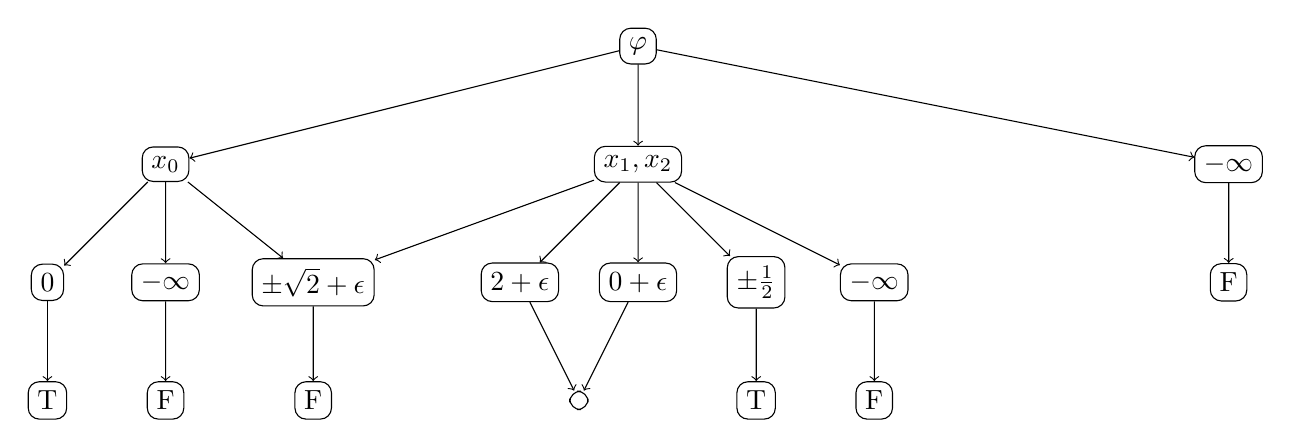
\begin{tikzpicture}[scale=1.5, 
				    state/.style={draw, rounded corners, fill=none,
				    			  text centered, text=black}]
	\node[state] (u1) at (5, 4) {$\varphi$};
	\node[state] (u2) at (1, 3) {$x_{0}$};
	\node[state] (u3) at (5, 3) {$x_{1},x_{2}$};
	\node[state] (u4) at (10, 3) {$-\infty$};
	\node[state] (u5) at (0, 2) {$0$};
	\node[state] (u6) at (1, 2) {$-\infty$};
	\node[state] (u7) at (2.25, 2) {$\pm\sqrt{2}+\epsilon$};
	\node[state] (u8) at (4, 2) {$2+\epsilon$};
	\node[state] (u9) at (5, 2) {$0+\epsilon$};
	\node[state] (u10) at (6, 2) {$\pm\frac{1}{2}$};
	\node[state] (u11) at (7, 2) {$-\infty$};
	\node[state] (u12) at (10, 2) {F};
	\node[state] (u13) at (0, 1) {T};
	\node[state] (u14) at (1, 1) {F};
	\node[state] (u15) at (2.25, 1) {F};
	\node[state] (u16) at (4.5, 1) {\lightning};
	\node[state] (u18) at (6, 1) {T};
	\node[state] (u19) at (7, 1) {F};

	
	\path[->] 	(u1)  edge   (u2);
	\path[->] 	(u1)  edge   (u3);
	\path[->] 	(u1)  edge   (u4);
	\path[->] 	(u2)  edge   (u5);
	\path[->] 	(u2)  edge   (u6);
	\path[->] 	(u2)  edge   (u7);
	\path[->] 	(u3)  edge   (u7);
	\path[->] 	(u3)  edge   (u8);
	\path[->] 	(u3)  edge   (u9);
	\path[->] 	(u3)  edge   (u10);
	\path[->] 	(u3)  edge   (u11);
	\path[->] 	(u4)  edge   (u12);
	\path[->] 	(u5)  edge   (u13);
	\path[->] 	(u6)  edge   (u14);
	\path[->] 	(u7)  edge   (u15);
	\path[->] 	(u8)  edge   (u16);
	\path[->] 	(u9)  edge   (u16);
	\path[->] 	(u10)  edge   (u18);
	\path[->] 	(u11)  edge   (u19);
\end{tikzpicture}

	\end{center}
	\caption{Example of Virtual Substitution.}
	\label{fig:graph}
\end{figure}